\chapter{Методология и архитектура}
\label{chap:met}

\section{Интеграция копилятора}
\label{sec:met:ls_compiler_interop}
Идея Языкового Сервера заключается в том, чтобы запускать экземпляр ЯС в том же каталоге проекта, который открыт в редакторе, и в подключении его к редактору по протоколу ЯС.

Языковой сервер отвечает за реализацию функций редактора по работе с кодом, он оперирует над семантическим представлением языка и другими метаданными, 
нужными для осуществения семантического анализа и, следовательно, предоставляет редактору данные в согласованном формате через протокол языкового сервера. 
Поскольку языковой сервер в значительной степени полагается на современный компилятор, который предоставляет SR, 
нам нужно реализовать способ интеграции компилятора в языковой сервер и обеспечить их взаимодействие.

Это можно сделать двумя способами: либо использовать компилятор в качестве библиотеки, 
либо вызывать его в отдельном процессе, передавая компилятору требуемые аргументы командной строки.\ref{table:met:compiler_integration}
\begin{table}[H]
    \centering
    \begin{tabular}{|c|c|}
        \hline
        \textbf{вызов команды} & \textbf{подключение через API} \\
        \hline
        \makecell{более простая интеграция} & \makecell{сложная интеграция} \\
        \hline
        \makecell{ограниченное количество опций вызова} & \makecell{возможность выражать сложные \\стратегии интеграции} \\
        \hline
        \makecell{необходисомть в разборе формата} & \makecell{возможность обмениваться \\типами данных компилятора} \\
        \hline
        \makecell{необходимость реализации своего \\API обхода семантического представления} & \makecell{компилятор может экспортировать \\API обхода представления} \\
        \hline
        \makecell{необходимость описания типов данных \\компилятора в языковом сервере} & \makecell{компилятор может экспортировать \\внутренние типы данных} \\
        \hline
    \end{tabular}
    \caption{Сравнение методик интеграции компилятора в языковой сервер}
    \label{table:met:compiler_integration}
\end{table}

Поскольку компилятор SLang\cite{Zouev2017} не предоставляет API обхода AST или внутренних типов данных, большинство преимуществ, 
характерных для опции "подключение через API", не применимы в нашем случае. 
Кроме того, компилятор предоставляет стабильное семантическое представление в формате JSON, который, 
будучи стандартизированным текстомым форматом, может быть легко передан через канал операционной системы, такой как standard output\cite{TheOpenGroup1997}.

Таким образом, мы получаем ряд удобных свойств когда компилятор вызывается нашим языковым сервером как команда, к тому же
этот вариант легче реализовать как на стороне языкового сервера, так и на стороне компилятора. 
И поскольку мы не ограничены какой-либо функциональностью, которая требовала бы подключения компилятора через API, 
мы можем считать этот способ интеграции наиболее уместным в нашем случае и придерживаться его.\ref{fig:met:compiler_integration}
\begin{figure}[H]
    \centering
    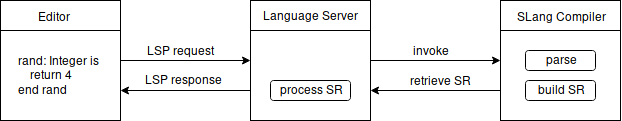
\includegraphics[width=1.0\textwidth]{figs/compiler_integration.png}
    \caption{Взаимодествие компилятора с языкомым сервером}
    \label{fig:met:compiler_integration}
\end{figure}

\section{Language Server Extensible Architecture}
\label{sec:met:arch}
The main idea of this research is to bring architecture of Language Servers to the next level,
make it modular and extensible, thus allowing third parties to throw in additional functionality for the SLang tooling
with no need to hack into the Language Server code.

Therefore, the architecture of the SLang Language Server is divided into two aggregate components: \ref{fig:met:ls_highlevel_arch}
\begin{itemize}
    \item The Core
    \item Module System
\end{itemize}

\begin{figure}[H]
    \centering
    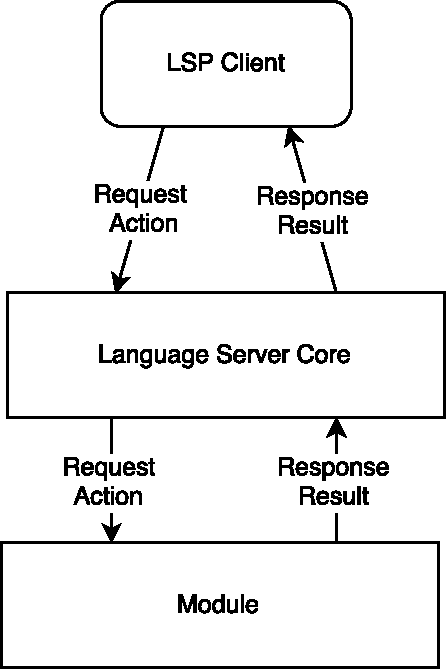
\includegraphics[width=.3\textwidth]{figs/highlevel_architecture.pdf}
    \caption{Language Server High-level Architecture}
    \label{fig:met:ls_highlevel_arch}
\end{figure}

\subsection{Language Server Core}
\label{sec:met:arch:core}
Language Server Core is a basement level of the Language Server on which Language Server Modules will operate.
Responsibilities of LS Core include:
\begin{itemize}
    \item LS Client connection maintenance
    \item Module registry maintenance
    \item Routing of incoming requests and data control flow between modules
\end{itemize}

Each of these responsibilities we shall describe in detail below.

\subsubsection{Client connection maintenance}
\label{sec:met:arch:core:connection_maintenance}
According to the Language Server Protocol\cite{Sourcegraph}, the client controls the lifetime of a server,
i.e starts it and shuts the server down on demand. After startup, the client connects to the server
using one of the transports. Since the transport level is not constrained by the LSP, specific transport can vary in different implementations.

Language Server Core should support several types of transport and be able to operate on them to accept requests and respond to the client. The list of widely used transports we are going to implement is
\begin{itemize}
    \item stdin/stdout
    \item TCP
    \item UDP
\end{itemize}
Implementing that list will supply the most of LSP clients with an option of how to work with the SLang Language Server.

\subsubsection{Module Registry}
\label{sec:met:arch:core:module_registry}

To be a foundation for an extensible modular architecture Language Server Core needs to have a subsystem
for module registering, maintenance and inter-operation organization.

\begin{figure}[H]
    \centering
    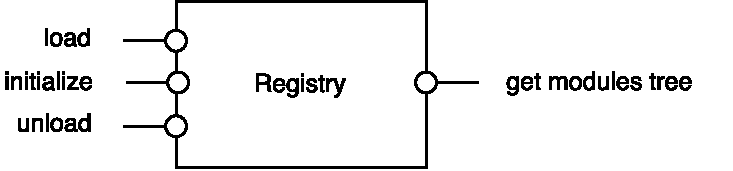
\includegraphics[width=.7\textwidth]{figs/registry.pdf}
    \caption{Module Registry API}
    \label{fig:met:registry_methods}
\end{figure}

\newpage
The registry should register a module and share its status, as well as information on how to launch and connect
internal (core) and external modules. On startup, the registry should initialize its state using a predefined directory
containing configuration files. Afterwards, it should maintain an API to load and unload additional modules via LSP.
Consequently, we need to extend the LSP with additional commands for the modules registry:\ref{fig:met:registry_methods}

\begin{itemize}
    \item registryCtl/load: register the module.
    \item registryCtl/unload: unregister the module.
    \item registryCtl/status: query module status.
\end{itemize}

\subsubsection{Dispatcher and data flow control}
\label{sec:met:arch:core:dispatcher}

After startup, connection setup, module registering and initialization,
the Language Server accepts the first request from the client.
This request gets validated by the Language Server Core, and then, after looking up the Module Registry, the request
gets handed over to the beginning of a processing pipeline responsible for handling this type of requests.

The dispatcher part is basically a glue, that connects all Language Server components together and
maintains the data flow edges of the modules graph, enabling module inter-operation by the
rules loaded into the Registry, that are discussed further in the section \ref{sec:met:arch:ms}.

There is a simpler alternative approach to module inter-operation organization: let the modules send data to each other and organize pipeline as they want.
Although this peer-to-peer schema here would save a lot of bandwidth, it would also inevitably lead to the dependency hell,
as such an approach would require having every module knowing about each other and to be connected to each other.
Thus, here we face the classic client/server trade-off: we can offload a ``server" (LS Core) only
if we complicate a ``client" (modules).
Since the client side is to be developed by third parties, the simpler it is -- the better:
the server, controlling all the data flow, will leave the module developer only with the business logic implementation tasks.

\subsection{Module System}
\label{sec:met:arch:ms}

Language Server is a great idea that enables IDE-like functionality for
comparably simple text editors, but currently these are mostly designed as
a monolithic software, while their service functions are naturally extensible,
e.g. it is common for a static analyzer to have modules for different diagnostics,
and similarly one of Language Server functions is to provide an editor with diagnostics, so here we can
have a hierarchy of at least two modules -- the compiler diagnostics and the diagnostics provided by an external static analysis tool.
We can go even further and implement a static analyzer as a combination of the base static analysis module with a bunch of atomic diagnostic modules derived from this base module.
The same logic is applicable to every Language Server service to some extent.

Separation of the monolithic core from the actual functionality implemented through modules
will significantly lower the Language Server internal bonding, and will make
module implementation relying on as stable API as possible, therefore allowing the core and modules
development to be performed simultaneously with no mutual API breakages.

Therefore another benefit of an extensible architecture that we can derive is the
Language Server easy adoption for any specific corporate needs.
As implementing some additional functionality would be as easy as developing a plug-in using
the Language Server Modules API, corporate users can extend the Language Server
according to their specific requirements, i.e add custom diagnostics, enforce code style,
or even hook-up the proprietary static analysis or code generation tools.

\begin{figure}[H]
    \centering
    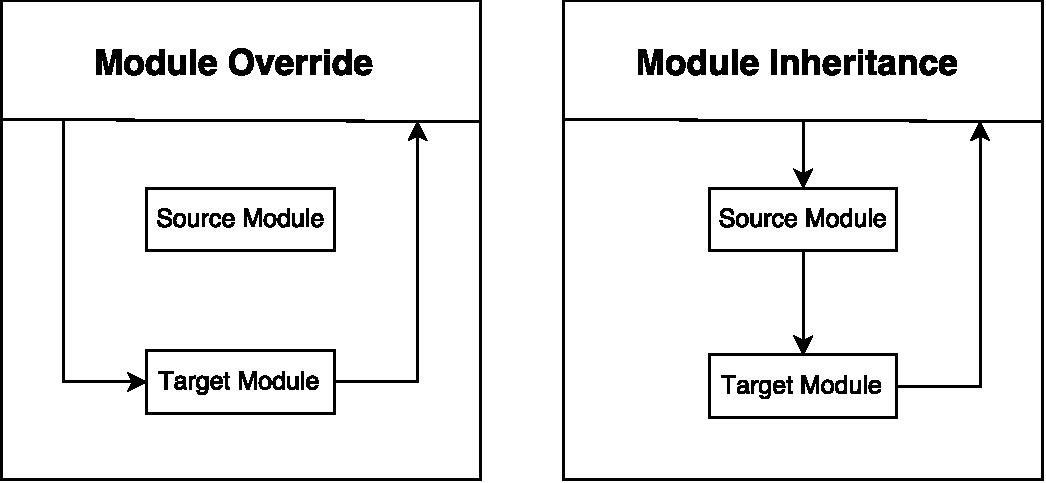
\includegraphics[width=.7\textwidth]{figs/module_hierarchy.pdf}
    \caption{Module Hierarchy}
    \label{fig:met:module_hierarchy}
\end{figure}

One of the ways to develop such architecture has already been introduced above: the hierarchy of modules expressed with the basic Object-Oriented Programming terms\ref{fig:met:module_hierarchy}.
In this hierarchy, modules can either override other modules or extend them in a way of post-processing the
results of the base module computation. So the modules would form a classic tree, deriving from a base module,
and intercepting the data flow. The example of such a module hierarchy is illustrated in the figure \ref{fig:met:module_tree}

\begin{figure}[H]
    \centering
    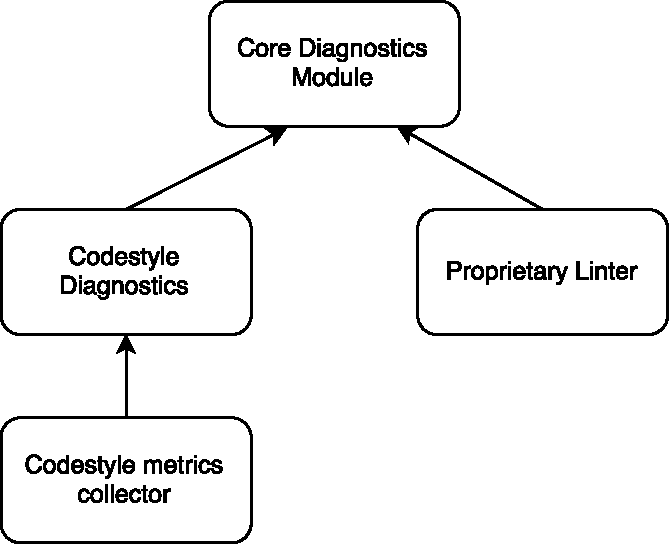
\includegraphics[width=.5\textwidth]{figs/module_tree.pdf}
    \caption{Example Modules Tree}
    \label{fig:met:module_tree}
\end{figure}

We already mentioned the hierarchy of the base and derived modules above. Taking the modern Object-Oriented languages`
type systems as an example, we can build a system with the base modules, which are to be deployed bundled with the Language Server and responsible for
one particular LS Protocol method each. These modules will mainly provide the basic runtime for all the derived modules:
\begin{itemize}
    \item set up data types: the input information, analysis context, and the results.
    \item perform the construction of the context (if applicable).
    \item intercept analysis results of the derived module and send them to the client through LSP.
\end{itemize}

As one could have figured, it is not really a conventional O-O paradigm inheritance model: core modules do not let the derived ones to override their logic as they work with the Language Server Client and therefore
are forced to live within the same process with the Language Server due to resources sharing. The process of a modular Language Server operation is showed on the sequence diagram \ref{fig:met:modules_sd}.

Hereby, we have two types of modules:
\begin{itemize}
    \item Core Modules: embedded into the LS process, exposing the run-time for external modules, cannot be overridden.
    \item External Modules: pluggable things, derived from the core modules, can be overridden.
\end{itemize}

\begin{figure}[H]
    \centering
    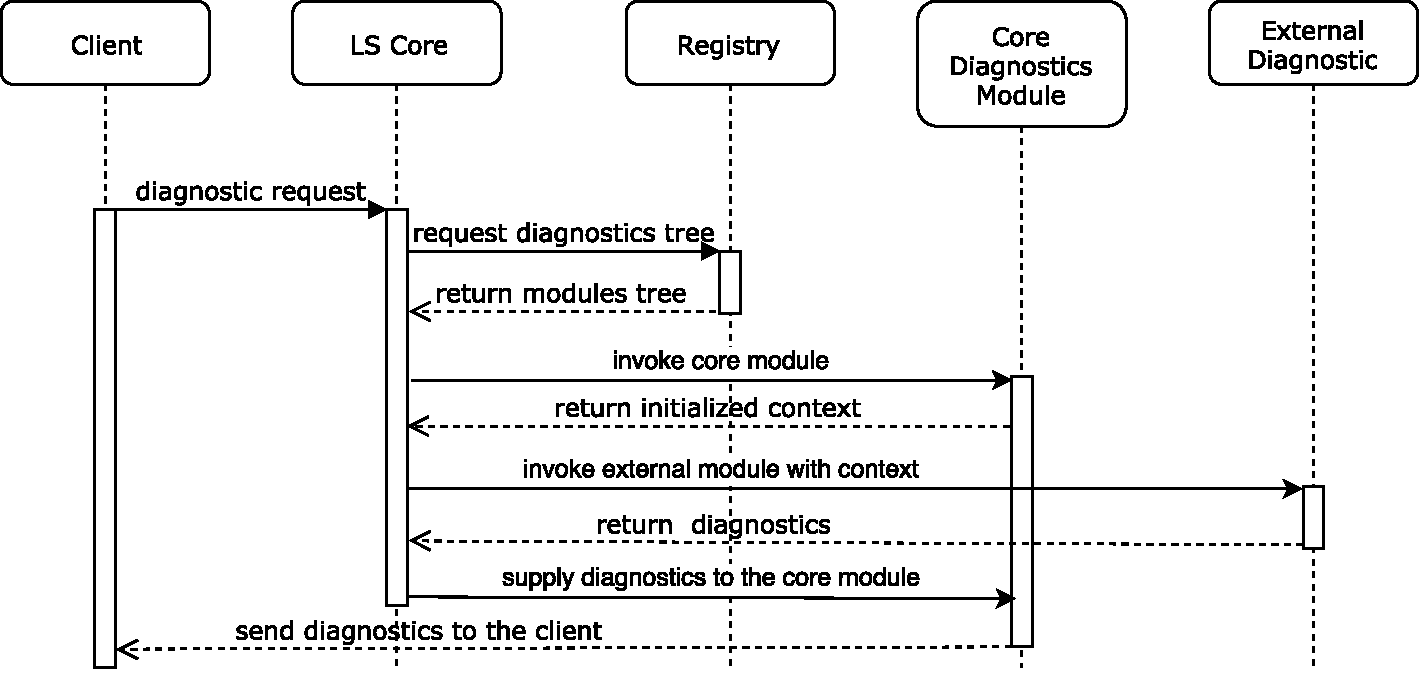
\includegraphics[width=1.0\textwidth]{figs/modules_sd.pdf}
    \caption{Modules invocation sequence diagram}
    \label{fig:met:modules_sd}
\end{figure}

Summing up, now we have a way to integrate the compiler into the Language Server, powerful extensible architecture that allows to throw in additional functionality for the Language Server, and modules hierarchy to start designing the core modules for the Language Server Protocol methods, as well as the external ones to perform actual analysis and supply Language Server Clients with the source code insights.

\section{Development Plan}
To implement a complex system it is vital to split the work into phases and introduce
the iterative development plan, that would cover a small self-contained part of work on each iteration,
in such a way that the result of each iteration could be presented as a working product.

Also, each iteration should include unit and integration testing to form good test coverage
at the end of the development and to simplify the process of project evolution through use of regression testing.

\textbf{A Dummy Language Server} \\
At first, the very basic functionality should be implemented: accepting the connection and handling a request with a hardcoded response

\textbf{SR-driven Language Server}\\
The next step would be to integrate the compiler and the language Semantic Representation
to feature ``jump to definition" for the SLang Language Server.

\textbf{Basic Modular Language Server}\\
After all the groundwork with the protocol and compiler inter-operation,
modular architecture implementation may be started: without foreign process extensions for now,
including only built-in modules, that operate in the same address space with the Language Server,
and the simple registry for them, to mock the basement for the future extensible LS.

\textbf{Extensible Language Server}\\
Finally, the last step is to extend the registry so it would handle configuration files
and load external modules and to extend the inner protocol and API to work with modules that are operating
in external processes, thus completing the extensible Language Server implementation for SLang.
The final architecture after this stage is illustrated in the figure \ref{fig:met:final_architecture}

\begin{figure}[H]
    \centering
    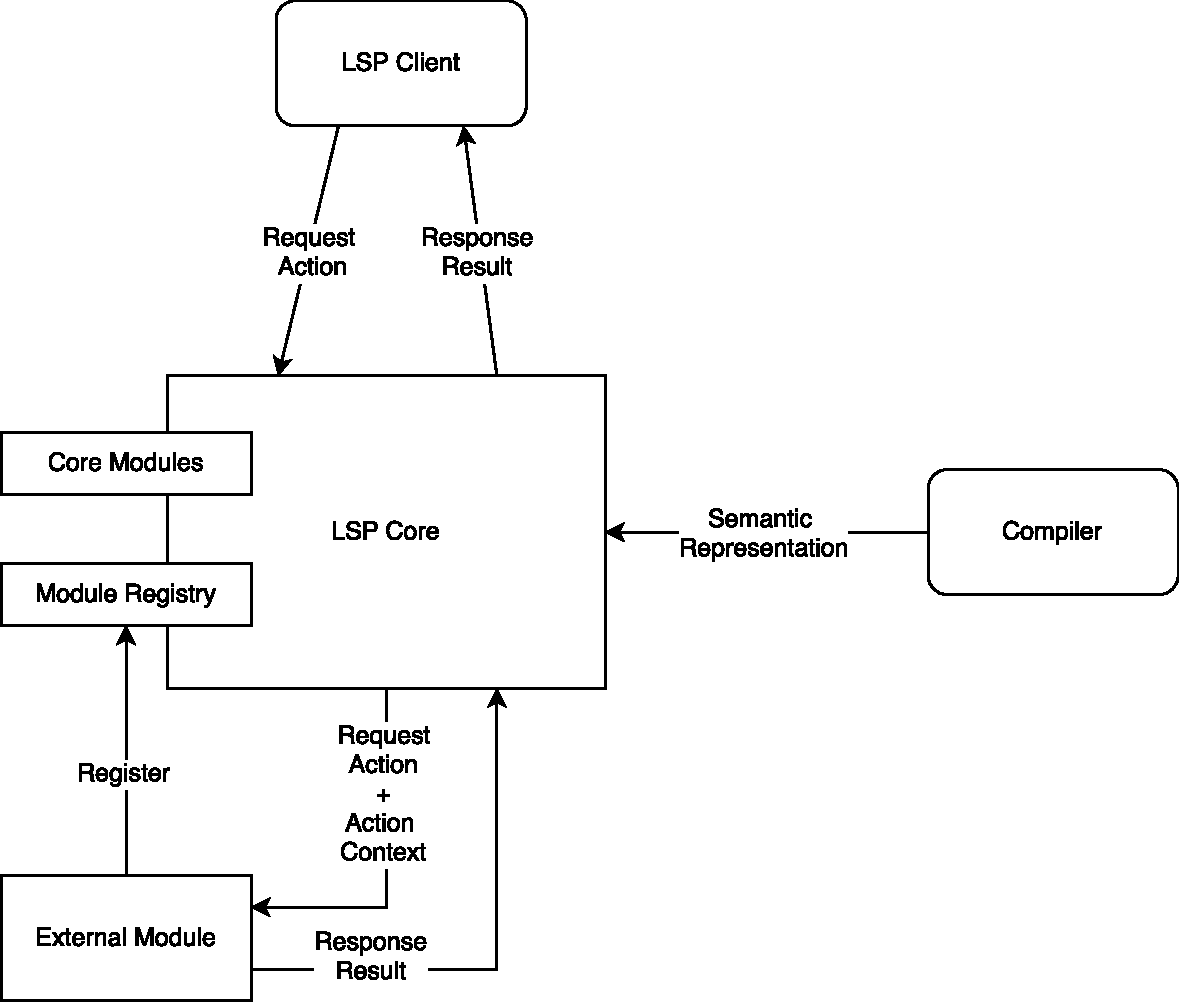
\includegraphics[width=.55\textwidth]{figs/ls_iteration_4.pdf}
    \caption{Final architecture}
    \label{fig:met:final_architecture}
\end{figure}

\newpage

\section{Approaches to implementations}

The most of the Language Server functionality heavily relies on the language`s semantic representation.
For the first prototype we are going to be using the SLang semantic representation and will build a few tools for it.

The SLang is using a json-formated SR with an object hierarchy described in the following section.

\subsection{SLang Semantic Representation format}

Slang has three scoping components: Unit, Block and Routine, where any nesting order is valid.
Each of these components has its context with encapsulated members as an array to
keep the consistent order:

\begin{lstlisting}
{
    "type": "Unit",
    "context": [
        {
            "type": "Routine",
            "context": [
                "type": "Block",
                "context": [
                    ...
                ]
            ]
        }
    ]
}
\end{lstlisting}

In addition to the described basic scoping hierarchy, SLang JSON SR unilizes some extra fields with
metadata and semantics extracted from the source code:

\begin{itemize}
    \item \textbf{name}: the program-specified name of a specific program entity (variable, routine, etc.), optional.
    \item \textbf{id}:   unique entity identifier, used for SR internal referencing.
    \item \textbf{ref}:  internal SR reference to an \textbf{id}, used for referencing the parent unit, variable definitions, etc.
    \item \textbf{span}: text locator of the entity containing the start and the end positions represented as a line:column pair.
    \item \textbf{signature}: the routine special case field containing the routine signature as input and output contexts.
\end{itemize}

The meaning of each of these fields is implementation-defined and their semantics rely on the entity type they are contained within.
For instance, for a \textbf{Unit} type, the \textbf{ref} field will be pointing to a parent \textbf{Unit},
and for a \textbf{Var} within an \textbf{Expr} entity the \textbf{ref} field will be a reference to this particular variable definition.
Thus we can avoid lengthy SR leaf definition in the Language Server code saving all the important semantics.

\subsection{Jump to definition}

The most basic developer tool as well as the most basic toolset part is a \textbf{jump to definition} command.
Basically it helps the developer to instantly open the file and the line with the definition of some code entity used in the source code.

To implement this part of the Language Server via analysis of SR, only three of its components are necessary:

\begin{itemize}
    \item \textbf{id}:   every definition inherently has its own unique identifier.
    \item \textbf{ref}:  every usage of an entity defined somewhere references the original definition by its id.
    \item \textbf{span}: knowing the id, the location of the definition can be found.
\end{itemize}

\subsection{Code completion}

Another very common instrument in a developer toolbox is autocompletion, provided by an IDE.
In our case the provision of an autocompletion is on the Language Server.

The most usual case of autocompletion usage is navigation among the encapsulated class (or \textbf{Unit}) members, where autocompletion
can provide user with the useful suggestions on the names of these members and their types.
Using the recursive \textbf{jump to definition} search, we can find a scope with the members to be suggested, read theit metadata
and present it to a user in a readable format.

% \section{Basic Language Server Modules}
% \label{sec:met:mods}
% \subsection{Code Semantic Based Highlights Module}
% \label{sec:met:mods:highlights}
% Architecture and methods of IR analysis for highlights

% Mapping from semantic entities to LSP highlighting staff

% \subsection{Autocomplete Module}
% \label{sec:met:mods:autocomplete}
% Description if autocomplete algorithms and data structures choice